\begin{frame}[fragile]                                                                                                                        
   \frametitle{Feeding AIL with custom JSON}
        \begin{itemize}
                \item AIL - feeder from Twitter\footnote{\url{https://github.com/ail-project/ail-feeder-twitter}}
                \item The AIL-feeder-twitter search in Twitter using Twint (without API), crawls the urls and pushes the results in AIL
                \item The JSON format format can be extended via meta fields
        \end{itemize}
\end{frame}

\begin{frame}[fragile]
	\frametitle{Feeding AIL with custom JSON}
	\begin{figure}[t]
		
\includegraphics[width=.8\textwidth]{screenshot/contileaks-twitter.png}
		\centering
	\end{figure}

	\begin{figure}[t]
		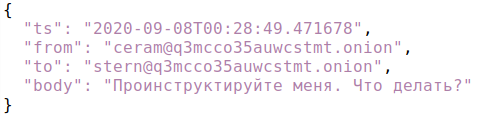
\includegraphics[width=.6\textwidth]{screenshot/contileaks-json.png}
		\centering
	\end{figure}

\end{frame}

\begin{frame}[fragile]                                                                                                                        

   \frametitle{Feeding AIL with custom JSON}

        \begin{itemize}
		\item Good candidate for AIL analysis:
        	\begin{itemize}
			\item PGP keys
			\item bitcoins addresses, maybe others,
			\item onion hidden services
        	\end{itemize}
                \item first we translated the files on english using deepl.com 
		\item modified AIL to interpret jabber ids as usernames,
		\item then we created a feeder to import json data in AIL
        \end{itemize}

\end{frame}


\begin{frame}[fragile]                                                                                                                        
   \frametitle{Feeding AIL with custom JSON}
	\lstinputlisting[language=Python]{feeder.py}

	\begin{lstlisting}[language=bash]
	$ cat ~/conti/* | jq . -c | python ./feeder.py
	\end{lstlisting}

\end{frame}

\begin{frame}[fragile]                                                                                                                        

   \frametitle{Feeding AIL with custom JSON}

        \begin{itemize}
		\item use grep to limit the noise on an instance by only sending interesting bits:
        	\begin{itemize}
			\item PGP keys
	\begin{lstlisting}[language=bash]
	$ cat ~/conti/* | jq . -c | grep PGP | python ./feeder.py
	\end{lstlisting}
			\item onion hidden services \texttt{| grep http:// |}
			\item telegram addresses \texttt{| grep tg:// | }
			\item bitcoins addresses \texttt{| egrep --regexp="[13][a-km-zA-HJ-NP-Z1-9]{25,34}" | }

        	\end{itemize}
        \end{itemize}

\end{frame}
